
\documentclass[11pt, class=report,crop=false]{standalone}
\usepackage[screen]{../exo7book}


\begin{document}

%====================================================================
\chapitre{Gradient -- Théorème des accroissements finis}
%====================================================================

% A garder
%\DeclareMathOperator{\grad}{grad}  % dans le préambule
\newcommand{\grad}{\operatorname{grad}} % dans le document


Le calcul différentiel s'applique au calcul des équations des tangentes aux courbes et des plans tangents aux surfaces.
Il permet aussi d'approcher les fonctions de plusieurs variables par des formules linéaires.


%%%%%%%%%%%%%%%%%%%%%%%%%%%%%%%%%%%%%%%%%%%%%%%%%%%%%
\section{Gradient}

Le gradient est un vecteur dont les coordonnées sont les dérivées partielles. 
Il est très important en physique et a des nombreuses applications géométriques, car il indique la direction perpendiculaire aux courbes et surfaces.

%----------------------------------------------------
\subsection{Rappel de la définition}

\begin{definition}
Soit $f : \Rr^n \to \Rr$ une fonction admettant des dérivées partielles.
Le \defi{gradient} en $x = (x_1,\ldots,x_n) \in \Rr^n$, noté 
$\grad f (x)$, est le vecteur 
$$\grad f (x) =
\begin{pmatrix} \dfrac{\partial f}{\partial x_{1}} (x)\\ \vdots \\ \dfrac{\partial f}{\partial x_n}(x)\end{pmatrix}.$$
\end{definition}

Les physiciens notent souvent $\nabla f (x)$ pour $\grad f (x)$.
Le symbole $\nabla$ se lit \og{}nabla\fg{}.

\bigskip

Pour une fonction $f(x,y)$ de deux variables, au point $(x_0,y_0)$, on a donc
$$\grad f(x_0,y_0) = \begin{pmatrix}  \dfrac{\partial f}{\partial x} (x_0,y_0) \\ \dfrac{\partial f}{\partial y}(x_0,y_0)\end{pmatrix}.$$


\begin{exemple}
\sauteligne
\begin{itemize}
\item Si $f(x,y) = x^2y^3$ alors $\grad f (x,y) =  \begin{pmatrix}2xy^3\\3x^2y^2\end{pmatrix}$.
Au point $(x_0,y_0)=(2,1)$, on a $\grad f (2,1) =  \begin{pmatrix}4\\12\end{pmatrix}$.

\item Si $f(x,y,z) = x^2\sin(yz)$ alors $\grad f (x,y,z) = \begin{pmatrix} 2x\sin(yz) \\ x^2z \cos(yz) \\ x^2y\cos(yz) \end{pmatrix}$.

\item Si $f(x_1,\ldots,x_n)= x_1^2+x_2^2+\cdots + x_n^2$ alors $\grad f (x_1,\ldots,x_n) =  \begin{pmatrix}2x_1\\ \vdots \\2x_n\end{pmatrix}$.
\end{itemize}
\end{exemple}

\begin{remarque*}
Le gradient est un élément de $\Rr^n$ écrit comme un vecteur colonne. C'est la transposée de la matrice jacobienne qui est ici un vecteur ligne. Parfois, pour alléger l'écriture, on peut aussi écrire le gradient sous la forme d'un vecteur ligne.
\end{remarque*}


%----------------------------------------------------
\subsection{Rappel du lien avec la différentielle}


\evidence{Lien avec la différentielle.}

Le gradient est une autre écriture possible de la différentielle.
Si $f$ est différentiable en $x \in \Rr^n$ et si $h \in \Rr^n$, alors :
\mybox{$\dd f (x) (h) = \langle \grad f (x) \mid h \rangle$}
où $\langle \cdot \mid \cdot \rangle$ désigne le produit scalaire.
Pour $f: \Rr^2 \to \Rr$ et $(x_0,y_0),(h,k) \in \Rr^2$, cela s'écrit :
$$\dd f (x_0,y_0) (h,k) = \langle \grad f (x_0,y_0) \mid \left(\begin{smallmatrix}h\\k\end{smallmatrix}\right) \rangle
= h\frac{\partial f}{\partial x}(x_0,y_0)
+k\frac{\partial f}{\partial y}(x_0,y_0).$$


La différentielle $\dd f(x)$ est une application linéaire de $\Rr^n$ dans $\Rr$ et $\grad f (x)$ est la transposée de sa matrice dans la base canonique.
On pourrait donc aussi écrire le produit de matrices $\dd f(x)(h) = \grad f (x)^T \cdot h$.

\bigskip

\evidence{Lien avec la dérivée directionnelle.}

Si $f$ est différentiable en $x \in \Rr^n$ et si $v \in \Rr^n$, alors :
$$D_v f(x) = \dd f (x) (v) = \langle \grad f (x) \mid v \rangle.$$



%----------------------------------------------------
\subsection{Tangentes aux lignes de niveau}


Soit $f : \Rr^2 \to \Rr$ une fonction différentiable et soit $k \in \Rr$. On considère les lignes de niveau $f(x,y)=k$, c'est-à-dire l'ensemble des $(x,y) \in \Rr^2$ qui vérifient l'équation $f(x,y)=k$.


\begin{proposition}
Le vecteur gradient $\grad f(x_0,y_0)$ est orthogonal à la ligne de niveau de $f$ passant au point $(x_0,y_0)$. 
\end{proposition}


Sur ce premier dessin, vous avez \couleurnb{(en rouge)}{} la ligne de niveau passant par le point $(x_0,y_0)$. En ce point est dessiné \couleurnb{(en vert)}{} un vecteur tangent $v$ et la tangente à la ligne de niveau. 
Le vecteur gradient \couleurnb{(en bleu)}{} est orthogonal à la ligne de niveau en ce point.


\bigskip

\myfigure{1}{
  \tikzinput{fig-gradient-02}
}

\bigskip

En chaque point du plan part un vecteur gradient. Ce vecteur gradient est orthogonal à la ligne de niveau passant par ce point.

\myfigure{1}{
  \tikzinput{fig-gradient-01}
}




Précisons la notion de tangente :
\begin{itemize}
  \item On se place en un point $(x_0,y_0)$ où les deux dérivées partielles ne s'annulent pas en même temps, c'est-à-dire $\grad f(x_0,y_0)$ n'est pas le vecteur nul. Considérons $\mathcal{C}$, la ligne de niveau de $f$ qui passe par ce point $(x_0,y_0)$. Le théorème des fonctions implicites (qui sera vu plus tard) montre qu'il est possible de trouver une paramétrisation de $\mathcal{C}$ au voisinage de $(x_0,y_0)$. Notons $\gamma : [-1,1] \to \Rr^2$, $t \mapsto \gamma(t)= (\gamma_1(t),\gamma_2(t))$ cette paramétrisation, en supposant que $\gamma(0) = (x_0,y_0)$. 


  \item La \defi{tangente} à la courbe $\mathcal{C}$ en $(x_0,y_0)$ est la droite passant par le point $(x_0,y_0)$ et de vecteur directeur le vecteur dérivé $\gamma'(0) = (\gamma_1'(0),\gamma_2'(0))$.
  
  \item Un vecteur $v$ est \defi{orthogonal} (ou \defi{normal} si $v$ n'est pas nul) à la courbe $\mathcal{C}$ en $(x_0,y_0)$ s'il est orthogonal à la tangente en ce point, c'est-à-dire si $\langle v \mid \gamma'(0)\rangle = 0$.
\end{itemize}

On peut maintenant prouver la proposition.
\begin{proof}
Notons $k = f(x_0,y_0)$. Alors $\mathcal{C}$ est la ligne de niveau $f(x,y)=k$.
Dire que $\gamma(t)$ est une paramétrisation de $\mathcal{C}$ (autour de $(x_0,y_0)$), 
c'est exactement dire que :
$$\forall t \in [-1,1] \qquad f \big( \gamma(t) \big) = k$$
Comme $f \circ \gamma$ est une fonction constante, alors sa dérivée est nulle.
La formule de la différentielle d'une composition s'écrit 
$$J_f (\gamma(t)) \times J_\gamma (t) = 0$$
et donc ici 
$$
\begin{pmatrix}
\frac{\partial f}{\partial x} (\gamma(t)) & 
\frac{\partial f}{\partial y} (\gamma(t)) \\
\end{pmatrix}
\times
\begin{pmatrix}
\gamma_1'(t)\\
\gamma_2'(t)
\end{pmatrix}
= 0.$$
En $t=0$, on trouve exactement 
$$\langle \grad f(x_0,y_0) \mid \gamma'(0) \rangle = 0,$$
ce qui signifie que le gradient est orthogonal au vecteur tangent.
\end{proof}


Dans la pratique, c'est l'équation de la tangente qui nous intéresse :

\begin{proposition}
L{'}équation de la tangente à la ligne de niveau de $f$ en $(x_0,y_0)$ est 
\mybox{$\displaystyle
\frac{\partial f}{\partial x}(x_0,y_0)(x-x_0)+\frac{\partial f}{\partial y}(x_0,y_0)(y-y_0)=0
$}
pourvu que le gradient de $f$ en ce point ne soit pas le vecteur nul.
\end{proposition}

\begin{proof}
C'est l'équation de la droite dont un vecteur normal est $\grad f(x_0,y_0)$ et qui passe par $(x_0,y_0)$.
\end{proof}


\begin{exemple}[Tangente à une ellipse]
Trouvons les tangentes à l'ellipse $\mathcal{E}$ d'équation $\frac{x^2}{a^2}+\frac{y^2}{b^2} = 1$ (avec $a,b>0$).

\myfigure{0.8}{
  \tikzinput{fig-gradient-03}
}


\begin{itemize}
  \item \textbf{Par les lignes de niveau.} 
  
  Cette ellipse $\mathcal{E}$ est la ligne de niveau $f(x,y)=1$ de la fonction
  $f(x,y) = \frac{x^2}{a^2}+\frac{y^2}{b^2}$. 
  Les dérivées partielles de $f$ sont :
  $$\frac{\partial f}{\partial x}(x_0,y_0) = \frac{2x_0}{a^2} \qquad
\frac{\partial f}{\partial y}(x_0,y_0) = \frac{2y_0}{b^2}$$
  Donc l'équation de la tangente à l'ellipse $\mathcal{E}$ en un de ces points $(x_0,y_0)$ est
  $$\frac{2x_0}{a^2}(x-x_0)+\frac{2y_0}{b^2}(y-y_0)=0.$$
  Mais comme $\frac{x_0^2}{a^2}+\frac{y_0^2}{b^2} = 1$ alors l'équation de la tangente se simplifie en $\displaystyle \frac{x_0}{a^2}x + \frac{y_0}{b^2} y = 1$.
  
  \item \textbf{Par une paramétrisation.}
  
  Une autre approche est de paramétrer l'ellipse $\mathcal{E}$ par 
  $\gamma(t) = (a \cos t, b \sin t)$, $t \in [0,2\pi[$.
  Le vecteur dérivé étant $\gamma'(t) = (-a \sin t, b \cos t)$, la tangente
  en $\gamma(t)$ est dirigée par le vecteur $(-b \cos t,-a \sin t)$.
  L'équation de la tangente en $\gamma(t)$ est donc
  $$-b \cos t (x - a \cos t) -a\sin t (y - b\sin t) = 0.$$
  En posant $x_0 = a \cos t$ et $y_0 = b \sin t$, on retrouve l'équation ci-dessus.

\end{itemize}
\end{exemple}

\begin{exemple}
Soit $f(x,y) = x^3-y^2-x$.
Nous allons calculer l'équation des tangentes aux courbes de niveau de $f$.

\begin{itemize}
  \item \textbf{Calcul du gradient.}  
  $\grad f(x,y) = \begin{pmatrix} 3x^2-1 \\ -2y \end{pmatrix}$.
  
  \item \textbf{Points où le gradient s'annule.} 
  $P_1 = \left( -\frac{\sqrt 3}{3},0 \right)$, $P_2 =\left( +\frac{\sqrt 3}{3},0 \right).$
  
  On calcule $f(P_1) = +\frac{2\sqrt3}{9}$, $f(P_2) = -\frac{2\sqrt3}{9}$. Ainsi $P_1$ est sur la ligne de niveau $f(x,y) = +\frac{2\sqrt3}{9}$ et $P_2$ sur celle $f(x,y) = -\frac{2\sqrt3}{9}$.
   
  \item \textbf{\'Equation de la tangente.}  
  En dehors de ces deux points, les courbes de niveau ont une tangente.
  Au point $(x_0,y_0)$, l'équation est 
  $$(3x_0^2-1)(x-x_0) -2y_0(y-x_0) = 0.$$
\end{itemize}  


Voici quelques lignes de niveau de $f$.
Le point $P_1$ est le point isolé \couleurnb{du niveau rouge }{}et il n'y a pas de tangente en ce point. Le point $P_2$ est le point double \couleurnb{du niveau vert }{}et il n'y a pas de tangente en ce point (en fait on pourrait dire qu'il y a deux tangentes).




\begin{center}
  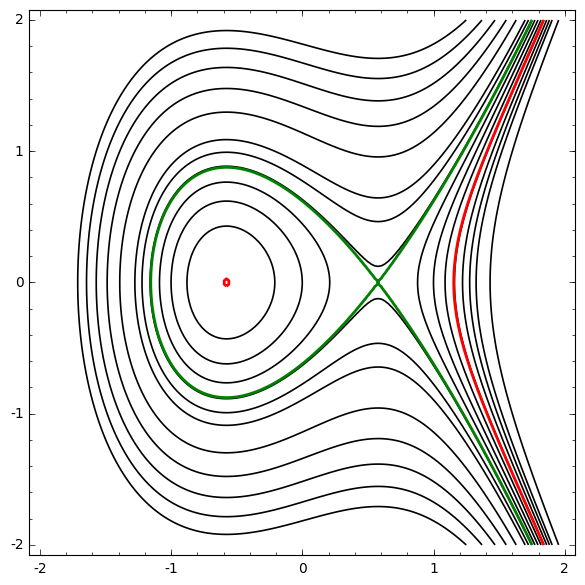
\includegraphics[scale=0.7]{figures/fig-gradient-04}
\end{center}

\end{exemple}






%----------------------------------------------------
\subsection{Lignes de plus forte pente}
 
Considérons les lignes de niveau $f(x,y)=k$ d'une fonction $f : \Rr^2 \to \Rr$.
On se place en un point $(x_0,y_0)$. On cherche dans quelle direction se déplacer pour augmenter le plus vite la valeur de $f$.
 
\begin{proposition}
Le vecteur gradient $\grad f(x_0,y_0)$ indique la direction de plus forte pente à partir du point $(x_0,y_0)$.
\end{proposition}


Autrement dit, si l'on veut passer le plus vite
possible du niveau $a$ à un niveau $b>a$, à partir d'un point donné $(x_0,y_0)$ de niveau
$f(x_0,y_0)=a$, alors il faut démarrer en suivant la direction du gradient $\grad f(x_0,y_0)$. 

\myfigure{1}{
  \tikzinput{fig-gradient-05}
}

Comme illustration, un skieur voulant aller vite choisit 
la plus forte pente descendante en un point de la montagne : c'est la direction opposée au gradient. 
 
\begin{proof}
La dérivée suivant le vecteur non nul $v$ au point $(x_0,y_0)$ décrit la variation de $f$ autour de ce point lorsqu'on se déplace dans la direction $v$. 
La direction selon laquelle la croissance est la plus forte est celle du gradient de $f$. En effet, on a 
$$D_{v}f(x_0,y_0)=\langle \grad f(x_0,y_0) \mid v\rangle=
\| \grad f(x_0,y_0) \| \cdot \| v \| \cdot \cos \theta$$
où $\theta$ est l'angle entre le vecteur $\grad f(x_0,y_0)$ et le vecteur $v$.
Le maximum est atteint lorsque l'angle $\theta$ est nul, c'est-à-dire lorsque $v$ pointe dans la même direction que $\grad f(x_0,y_0)$.
\end{proof}


%----------------------------------------------------
\subsection{Surfaces de niveau}

On a des résultats similaires pour les surfaces de niveau $f(x,y,z)=k$ d'une fonction $f$ différentiable.

Rappelons que le plan de $\Rr^3$ passant par $(x_0,y_0,z_0)$ et de vecteur normal 
$n=(a,b,c)$ a pour équation cartésienne :
$a(x-x_0)+b(y-y_0)+c(z-z_0)=0$.


De même qu'il existe une droite tangente à une ligne de niveau, il existe un \defi{plan tangent} à une surface de niveau.


\begin{proposition}
Le vecteur gradient $\grad f(x_0,y_0,z_0)$ est orthogonal à la surface de niveau de $f$ passant au point $(x_0,y_0,z_0)$. Autrement dit, l'équation du plan tangent à la surface de niveau de $f$ en $(x_0,y_0,z_0)$ est 
\mybox{$\displaystyle
\frac{\partial f}{\partial x}(x_0,y_0,z_0)(x-x_0)+\frac{\partial f}{\partial y}(x_0,y_0,z_0)(y-y_0)
+\frac{\partial f}{\partial z}(x_0,y_0,z_0)(z-z_0)=0
$}
pourvu que le gradient de $f$ en ce point ne soit pas le vecteur nul.
\end{proposition}


\myfigure{1}{
  \tikzinput{fig-gradient-07}
}


Plus généralement, pour $f : \Rr^n \to \Rr$, $\grad f (x_0)$ est orthogonal à l'espace tangent à l'hypersurface de niveau $f(x)=k$ passant par le point $x_0\in\Rr^n$.


\begin{exemple}
Pour quelles valeurs de $k$ la surface de niveau $x^2+y^2-z^2=k$ admet-elle un plan tangent horizontal (c'est-à-dire parallèle au plan $(z=0)$) ?

\emph{Solution.}
On pose $f(x,y,z) = x^2+y^2-z^2$.
\begin{itemize}
  \item \textbf{Calcul du gradient.}   
  $\grad f (x,y,z) = \begin{pmatrix}2x\\2y\\-2z\end{pmatrix}$.
  
  \item \textbf{Gradient nul.} Le gradient est le vecteur nul uniquement au point $(0,0,0)$, donc au niveau $k=0$. En ce point, il n'y a pas de plan tangent.
  
  \item \textbf{Plan tangent horizontal.}  
  Le plan tangent est horizontal exactement lorsque le gradient est un vecteur colinéaire à $\left(\begin{smallmatrix}0\\0\\1\end{smallmatrix}\right)$ (et n'est pas le vecteur nul).
  Il faut donc $\frac{\partial f}{\partial x} = 0$ et $\frac{\partial f}{\partial y} = 0$, ce qui implique ici $x=0$ et $y=0$.
  
  \item \textbf{Analyse.}
  En un tel point $(0,0,z)$, on a $f(x,y,z)=-z^2$, donc le niveau $k$ est strictement négatif.
  
  \item \textbf{Synthèse.} Réciproquement, étant donné $k<0$, alors aux points $(0,0,\pm\sqrt{|k|})$, le vecteur gradient est vertical, donc le plan tangent est horizontal.
  
  \item \textbf{Conclusion.}
  \begin{itemize} 
    \item Pour $k>0$, il n'y a pas de plan tangent horizontal. La surface $f(x,y,z)=k$ est un \defi{hyperboloïde à une nappe}. 
    
    \item Pour $k=0$, il n'y a pas de plan tangent horizontal. Le point $(0,0,0)$ est singulier. La surface $f(x,y,z)=0$ est un \defi{cône}. 
    
    \item Pour $k<0$, il y a deux points ayant un plan tangent horizontal. La surface $f(x,y,z)=k$ est un \defi{hyperboloïde à deux nappes}.   
    
    \end{itemize}
    
\end{itemize}  

De gauche à droite : l'hyperboloïde à une nappe, le cône, l'hyperboloïde à deux nappes.

\begin{center}
  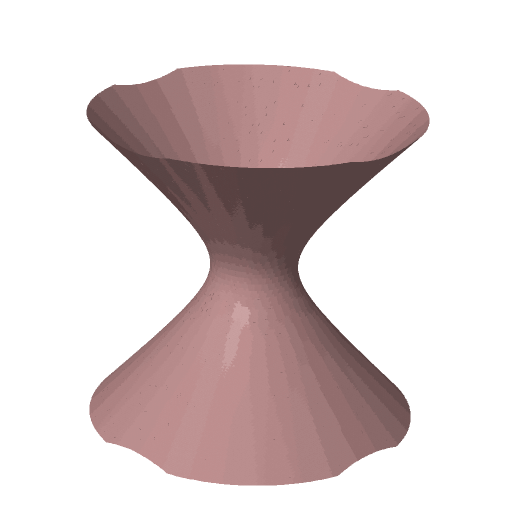
\includegraphics[scale=0.25]{figures/fig-gradient-06d}
  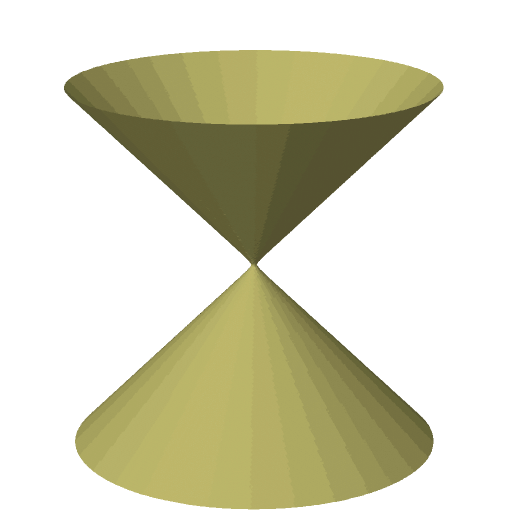
\includegraphics[scale=0.23]{figures/fig-gradient-06c}  
  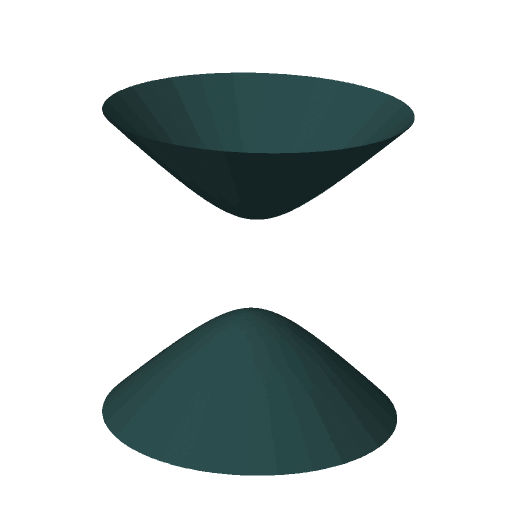
\includegraphics[scale=0.25]{figures/fig-gradient-06b}
\end{center}
Les trois surfaces ensemble, comme des surfaces de niveau de $f$ (avec une découpe pour voir l'intérieur). 
\begin{center}  
  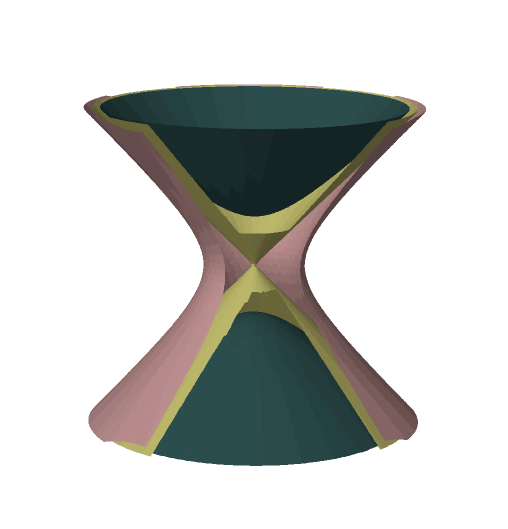
\includegraphics[scale=0.4]{figures/fig-gradient-06a}   
\end{center}
  
\end{exemple}

%--------------------------------------------------
\subsection{Plan tangent au graphe d'une fonction}

Soit $f : U \subset \Rr^2 \to \Rr$ différentiable.
On s'intéresse maintenant au graphe de $f$. Rappelons que c'est la surface
$$\mathcal{G}_f = \big\{ (x,y,z) \in \Rr^3 \mid (x,y)\in U \text{ et } z = f(x,y) \big\}.$$

Attention ! Il ne faut pas confondre le graphe d'une fonction $f : \Rr^2 \to \Rr$
avec les surfaces de niveau de fonctions $f : \Rr^3 \to \Rr$.


\begin{proposition}
Soit $f : U \subset \Rr^2 \to \Rr$ différentiable. Soit $(x_0,y_0) \in U$ et 
soit $M_0=(x_0,y_0,f(x_0,y_0))$ un point du graphe $\mathcal{G}_f$ de $f$.
Le plan tangent au graphe $\mathcal{G}_f$ en $M_0$ a pour équation :
\mybox{$\displaystyle 
z = f(x_0,y_0)+\frac{\partial f}{\partial x}(x_0,y_0)(x-x_0)
+\frac{\partial f}{\partial y}(x_0,y_0)(y-y_0)$}
\end{proposition}


\myfigure{1}{
  \tikzinput{fig-gradient-08}
}



\begin{proof}
On introduit la fonction $F$ définie par
$F(x,y,z)=z-f(x,y)$, pour tout $(x,y,z)\in U\times \Rr$.
Le graphe de $f$ est la surface $\mathcal{G}_f=\{(x,y,z)\in U\times \Rr\mid F(x,y,z)=0\}$.
Ainsi, $\mathcal{G}_f$ est aussi une surface de niveau de $F$.
On calcule : 
$$\grad F (x,y,z)=\left(-\frac{\partial f}{\partial x}(x,y),-\frac{\partial f}{\partial y}(x,y),1\right)$$
Notez que ce vecteur n'est jamais nul et donc une équation du plan tangent en $(x_0,y_0,z_0)$ est :
$$\frac{\partial f}{\partial x}(x_0,y_0)(x-x_0)
+\frac{\partial f}{\partial y}(x_0,y_0)(y-y_0) - (z-z_0) = 0$$
où on a noté $z_0 = f(x_0,y_0)$.
\end{proof}


\begin{exemple}
Soit $f(x,y) = 3x^2-2y^3$. 

\begin{enumerate}
  \item Trouver l'équation du plan tangent au graphe de $f$ au-dessus de $(x_0,y_0)$.
  
  On a $\frac{\partial f}{\partial x}(x,y) = 6x$, $\frac{\partial f}{\partial y}(x,y) = -6y^2$. Donc l'équation du plan tangent au point $(x_0,y_0,f(x_0,y_0))$ est :
  $$z = 3x_0^2-2y_0^3 + 6x_0(x-x_0) - 6y_0^2(y-y_0)$$
  ou encore
  $$6x_0x-6y_0^2y-z = 3x_0^2-4y_0^3.$$
  
  \item \emph{Application.} Trouver l'équation du plan $\mathcal{P}_0$ tangent au-dessus du point $(x_0,y_0)=(1,2)$.
  
  On pose $z_0 = f(x_0,y_0) =  -13$. L'équation est alors
  $z = -13 + 6(x-1)-24(y-2)$, autrement dit $6x-24y-z = -29$.
    
  \item Trouver les points pour lesquels le plan tangent est parallèle à $\mathcal{P}_0$.
  
  On cherche un point $(x_1,y_1)$ qui vérifie
  $(6,-24,-1) = (6x_1,-6y_1^2,-1)$  et $(x_1,y_1) \neq (x_0,y_0)$. On trouve comme seul autre point $(x_1,y_1)=(1,-2)$. 
  
\end{enumerate}

\end{exemple}

%----------------------------------------------------
\begin{miniexercices}
\sauteligne
\begin{enumerate}
  \item Calculer le gradient en tout point de la fonction définie par $f(x,y) = xe^y$. Même question pour $f(x,y,z) = x^2y^3z^4$, puis $f(x_1,\ldots,x_n)= \sqrt{x_1^2+\cdots+x_n^2}$. 
  
  \item  Calculer le gradient de $f(x,y) = \ln(x+y^2)$ en tout point $(x_0,y_0)$.
  Exprimer la différentielle $\dd f(x_0,y_0)(h,k)$. Calculer la dérivée directionnelle de $f$ en $(x_0,y_0)=(1,2)$ le long du vecteur $(2,3)$.
  
  \item Soient $f,g : \Rr^n \to \Rr$.
  Montrer que $\grad (f+g) (x) = \grad f(x) + \grad g(x)$. Que vaut $\grad (\lambda \cdot f) (x)$ (où $\lambda \in \Rr$) ?
  
  \item Trouver $f : \Rr^n \to \Rr$ et $x,y \in \Rr^n$ 
  tels que $\grad f (x+y)$ n'est pas égal à $\grad f (x) +\grad f (y)$.
  Trouver $f : \Rr^n \to \Rr$, $x \in \Rr^n$ et $\lambda \in \Rr$ tels que $\grad f (\lambda \cdot x)$ n'est pas égal à $\lambda \cdot \grad f (x)$.
     
  \item Soit l'hyperbole $\mathcal{H}$ d'équation $x^2-y^2=1$. Dessiner $\mathcal{H}$. Calculer l'équation cartésienne de la tangente en un point $(x_0,y_0) \in \mathcal{H}$. Trouver les points de $\mathcal{H}$ où la tangente est colinéaire au vecteur $(2,1)$.
   
  \item Trouver les points de la surface d'équation $x^2-y^2z=0$ où le gradient s'annule. Calculer l'équation du plan tangent en dehors de ces points.
  
  \item Soit $f(x,y) = \ln(x+y^2)$. Trouver l'équation du plan tangent au graphe de $f$ au-dessus du point $(-2,3)$.
  
   
  
\end{enumerate}
\end{miniexercices}



%%%%%%%%%%%%%%%%%%%%%%%%%%%%%%%%%%%%%%%%%%%%%%%%%%%%%
\section{Calcul d'incertitudes}

Pour les fonctions d'une variable, la dérivée permet de calculer un développement limité à l'ordre $1$ et donc d'approcher une fonction autour d'un point par une formule linéaire. Pour les fonctions de plusieurs variables, nous avons besoin des dérivées partielles pour obtenir une formule linéaire.

%----------------------------------------------------
\subsection{Calcul approché}

Motivation : comment estimer la valeur $\sqrt{1,01}$ sans calculatrice ?
On pose $f(x)=\sqrt{x}$. Le développement limité en $1$ s'écrit
$f(1+h) \simeq f(1) + hf'(1)$. Dans ce cas, on obtient :
$$\sqrt{1+h} \simeq 1 + \frac{h}{2}.$$
Cela donne l'estimation  $\sqrt{1,01} \simeq 1,005$ (au lieu de 
$\sqrt{1,01} = 1,00498\ldots$).

Géométriquement, la tangente au graphe de $f$ en $1$ donne une bonne approximation des valeurs de $f$ autour de ce point.

\myfigure{1}{
  \tikzinput{fig-gradient-09}
}
\bigskip

Nous allons voir l'analogue pour les fonctions de deux variables.

Si $f$ est différentiable au point $A = (x_0,y_0)$, alors
$$f(x_0+h,y_0+k) = f(x_0,y_0) + \dd f(x_0,y_0) (h,k) + o(\sqrt{h^2+k^2}).$$
On propose alors comme approximation de $f(x_0+h,y_0+k)$ la quantité 
$f(x_0,y_0) + \dd f(x_0,y_0) (h,k)$, appelée \defi{approximation linéaire}, c'est-à-dire :
\mybox{$\displaystyle
f(x_0+h,y_0+k) \simeq f(x_0,y_0) + h\frac{\partial f}{\partial x}(x_0,y_0)
+k\frac{\partial f}{\partial y}(x_0,y_0)
$}
C'est une approximation qui est valable pour $h$ et $k$ petits.

L'interprétation géométrique est la suivante : 
on approche le graphe de $f$ en $(x_0,y_0)$ par le plan tangent au graphe en ce point. Sur la figure ci-dessous sont représentés : le graphe de $f$\couleurnb{ (en rouge)}{}, le plan tangent au-dessus du point $(x_0,y_0)$\couleurnb{ (en bleu)}{}. La valeur $z_1 = f(x_0+h,y_0+k)$ est la valeur exacte donnée par le point de la surface au-dessus de $(x_0+h,y_0+k)$. On approche cette valeur par la valeur $z_2 = f(x_0,y_0) + h\frac{\partial f}{\partial x}(x_0,y_0)
+k\frac{\partial f}{\partial y}(x_0,y_0)$ donnée par le point du plan tangent au-dessus de $(x_0+h,y_0+k)$. 


\myfigure{1}{
  \tikzinput{fig-gradient-10}
}


\begin{exemple}
Valeur approchée de $f(1,002 ; 0,997)$ si $f(x,y) = x^2y$.
\bigskip

\emph{Solution.}
Ici, on a $(x_0,y_0) = (1,1)$, $h = 2 \times 10^{-3}$, $k = -3 \times 10^{-3}$,
$\frac{\partial f}{\partial x} = 2xy$, $\frac{\partial f}{\partial y} = x^2$, donc $\frac{\partial f}{\partial x}(x_0,y_0) = 2$, $\frac{\partial f}{\partial x}(x_0,y_0) = 1$. Ainsi, on a
$$f(1+h,1+k) \simeq f(1,1) + 2h + k$$
et donc 
$$f(1,002 ; 0,997) \simeq 1 + 2 \times 2 \times 10^{-3} - 3 \times 10^{-3} = 1,001.$$
Avec une calculatrice, on trouve $f(1,002 ; 0,997) = 1,000991988$ : l'approximation est bonne.
\end{exemple}

\begin{exemple}
Deux résistances $R_1$ et $R_2$ sont connectées en parallèle. La résistance totale $R$ du circuit est donnée par la formule 
$$\frac{1}{R} = \frac{1}{R_1} + \frac{1}{R_2}.$$

La résistance $R_1$ vaut environ $1$ ; $R_2$ vaut environ $2$ (en kilo-ohms).
\'Ecrire l'approximation linéaire correspondante, puis donner une valeur approchée de $R$ lorsque $R_1 = 1,01$ et $R_2 = 1,98$.

\bigskip

\emph{Solution.}
Notons $f(x,y) = \frac{1}{\frac{1}{x} + \frac{1}{y}} = \frac{xy}{x+y}$, de sorte que $R = f(R_1,R_2)$.
Par exemple, si $R_1 = 1$ et $R_2 = 2$, on trouve $R = 0,6666\ldots$


On calcule 
$$\frac{\partial f}{\partial x}(x,y) = \frac{y^2}{(x+y)^2} \qquad
\frac{\partial f}{\partial y}(x,y) = \frac{x^2}{(x+y)^2}.$$

Posons $(x_0,y_0)=(1,2)$. On a $f(x_0,y_0) = \frac 23$,
$\frac{\partial f}{\partial x}(x_0,y_0) = \frac 49$,
$\frac{\partial f}{\partial y}(x_0,y_0) = \frac 19$.

L'approximation linéaire de $f$ au voisinage de $(x_0,y_0)$ s'écrit
$$f(1+h,2+k) \simeq \frac 23 + \frac49 h + \frac19 k.$$
Avec $h = 0,01$ et $k = -0,02$, on obtient
$f(1,01 ; 1,98) \simeq 0,6689$.
\end{exemple}


%----------------------------------------------------
\subsection{Calcul d'incertitudes}


Soit $f(x,y)$ une grandeur qui dépend de deux mesures $x$ et $y$.
La valeur de $x$ est proche d'une valeur fixe $x_0$, mais n'est connue qu'à une incertitude près, c'est-à-dire $x \in [x_0-\Delta x,x_0 + \Delta x]$ où $\Delta x$ est un nombre réel positif, appelé l'\defi{incertitude} sur $x$.
De même, $y \in [y_0-\Delta y,y_0 + \Delta y]$.

Quelle va être l'erreur commise en approchant $f(x,y)$ par $f(x_0,y_0)$ ?



On note $(x,y) = (x_0+h,y_0+k)$. On a alors
$$
  \big| f(x_0+h,y_0+k) - f(x_0,y_0) \big| 
   \simeq \left| h\frac{\partial f}{\partial x}(x_0,y_0)
+k\frac{\partial f}{\partial y}(x_0,y_0) \right| 
   \le \Delta x \left|\frac{\partial f}{\partial x}(x_0,y_0) \right| 
+ \Delta y \left|\frac{\partial f}{\partial y}(x_0,y_0) \right| .
$$


On obtient ainsi une majoration de l'\defi{incertitude estimée} $\delta f$ :
$$\delta f \le \Delta x \left|\frac{\partial f}{\partial x}(x_0,y_0) \right| 
+ \Delta y \left|\frac{\partial f}{\partial y}(x_0,y_0) \right|$$


\begin{exemple}
Une usine produit des cylindres de rayon $r = 2 \pm 0,1$ et de hauteur $h = 10 \pm 0,2$. Quelle est l'incertitude estimée sur le volume du cylindre ?

\bigskip

\emph{Solution.}
Le volume est donné par la formule $V(r,h) = \pi r^2 h$.
On pose $r_0 = 2$, $\Delta r = 0,1$, $h_0 = 10$, $\Delta h = 0,2$.
Ainsi l'incertitude estimée vérifie
$$\delta V \le \Delta r\left|\frac{\partial V}{\partial r}(r_0,h_0) \right| + \Delta h\left|\frac{\partial V}{\partial h} (r_0,h_0)\right| .$$
On a 
$\frac{\partial V}{\partial r} = 2\pi r h$ 
et $\frac{\partial V}{\partial h} = \pi r^2$, donc ici :
$\delta V \le 0,1 \times 40\pi + 0,2 \times 4 \pi = 4,8\pi \simeq 15$.   
Le volume sans erreur est $V_0 = V(r_0,h_0) = 40 \pi \simeq 126$.
Au vu de notre estimation de l'incertitude, on écrit 
$$V(r,h) = 126 \pm 15.$$

\end{exemple}

\begin{remarque*}
Sur cet exemple, $r$ est ici connu avec une incertitude relative 
$\frac{\Delta r}{r_0} = \frac{0,1}{2} = 5\,\%$, et pour 
$h$ l'incertitude relative est $\frac{\Delta h}{h_0} = \frac{0,2}{10} = 2\,\%$.
L'estimation de l'incertitude relative du volume est 
$\frac{\delta V}{V_0} \simeq  \frac{15}{126} \simeq 12 \,\%$.
L'erreur relative du volume est donc bien plus élevée que les erreurs relatives sur $r$ et $h$.
\end{remarque*}

\begin{remarque*}
La formule de l'incertitude est seulement une estimation.
Pour une majoration exacte de l'erreur, il faut utiliser le théorème ou l'inégalité des accroissements finis.
\end{remarque*}


%----------------------------------------------------
\begin{miniexercices}
\sauteligne
\begin{enumerate}

  \item Donner l'approximation linéaire de $y^2e^x$ en $x_0=1$ et $y_0=2$. Sans calculatrice, en déduire une valeur approchée de $(1,99)^2 e^{1,03}$. Faire le même travail pour $\frac{\ln(9,99 \times 2,02)}{2,02}$.
  On admettra que $e \simeq 2,718$  et $\ln(20) \simeq 2,996$.
  
  \item La tension $U$, la résistance $R$ et l'intensité $I$ sont reliées par la loi d'Ohm $U = RI$. \'Ecrire l'approximation linéaire de la résistance, pour $U_0 = 120$ et $I_0 = 1$. Estimer la résistance lorsque $U = 118$ et $I = 0,9$.
  Estimer l'erreur commise lorsque l'on approche la résistance $R$ par $R_0 = U_0/I_0$ pour $U \in [118,122]$ et $I \in [0,9 ; 1,1]$.
  
  \item Soit $f(x,y) = \sqrt{x^2 + y^2}$. \'Ecrire l'approximation linéaire  pour $f(x,y)$ autour de $(x_0,y_0) = (4,3)$.
  Pour $x$ connu avec une incertitude relative de $5\,\%$ autour de $x_0$,
  et $y$ connu avec une incertitude relative de $10\,\%$ autour de $y_0$, estimer l'erreur relative commise lorsque l'on approche $f(x,y)$ par $f(x_0,y_0)$.
    
\end{enumerate}
\end{miniexercices}


%%%%%%%%%%%%%%%%%%%%%%%%%%%%%%%%%%%%%%%%%%%%%%%%%%%%%
\section{Théorème des accroissements finis}

Le théorème des accroissements finis est une façon exacte de mesurer l'écart entre deux valeurs de $f$. On peut aussi en tirer des inégalités. Cette section est beaucoup plus théorique que le reste du chapitre et peut être passée lors d'une première lecture.


%----------------------------------------------------
\subsection{Théorème des accroissements finis en une variable (rappel)}

\begin{theoreme}[Théorème des accroissements finis en une variable]
Soit $f:[a,b] \rightarrow \Rr$ continue sur $[a,b]$, dérivable sur $]a,b[$,  o\`u $a<b$. Il existe $c \in ]a,b[$ tel que
$$f(b)-f(a)=f'(c)(b-a).$$
\end{theoreme}
 
On renvoie au cours de première année pour la preuve.


%----------------------------------------------------
\subsection{Théorème des accroissements finis en deux variables}


\begin{theoreme}[Théorème des accroissements finis en deux variables]
Soit $f: U \to \Rr$ une fonction de classe $\mathcal{C}^1$ sur un ouvert $U \subset \Rr^2$. Soient $a,b$ deux points de $U$. Si le segment $[a,b]$ est inclus dans $U$, alors il existe 
$c \in ]a,b[$ tel que
$$f(b)-f(a) = \left\langle \grad f (c) \mid b-a \right\rangle.$$
\end{theoreme}


\'Enoncé ainsi, le théorème est valable aussi pour $U \subset \Rr^n$ ; en plus, en se souvenant que la différentielle s'exprime à l'aide du gradient $\dd f(c)(h) = \left\langle \grad f (c) \mid h \right\rangle$, on obtient une reformulation similaire au cas d'une variable : 
$$f(b)-f(a) = \dd f(c)(b-a)$$

Revenons au cas de deux variables et à une autre reformulation. Pour $\theta \in {}]0,1[$, on note
$$a = (x_0,y_0), \quad b=(x_0+h,y_0+k), \quad c = a+\theta (b-a) = (x_0+\theta h,y_0+\theta k) \in ]a,b[$$
et
$$\grad f (c) = 
\begin{pmatrix}
\dfrac{\partial f}{\partial x}(c) \\
\dfrac{\partial f}{\partial y}(c) \end{pmatrix} 
\qquad
b-a = \begin{pmatrix} h \\ k \end{pmatrix} .$$

\myfigure{0.7}{
  \tikzinput{fig-gradient-11}
}

\begin{theoreme}[Théorème des accroissements finis en deux variables]
Soit $f: U \to \Rr$ une fonction de classe $\mathcal{C}^1$ sur un ouvert $U \subset \Rr^2$ et soit $(x_0,y_0) \in U$. 
Pour tout $(h,k) \in \Rr^2$ tel que $(x_0+h,y_0+k)\in U$
et tel que $(x_0+th,y_0+tk)\in U$ pour tout $t\in[0,1]$, 
il existe $\theta \in ]0,1[$ tel que
$$f(x_0+h,y_0+k) - f(x_0,y_0) = 
h\frac{\partial f}{\partial x}(x_0+\theta h,y_0+\theta k)
+k\frac{\partial f}{\partial y}(x_0+\theta h,y_0+\theta k).$$
\end{theoreme}


\begin{exemple}
Soient $f(x,y) = e^{x-y^2}$, $a = (0,0)$, $b=(2,1)$.
\begin{itemize} 
  \item Le théorème des accroissements finis nous dit qu'il existe $c \in ]a,b[$ tel que 
$$f(b)-f(a) = \left\langle \grad f (c) \mid b-a \right\rangle.$$

  \item On a   $\frac{\partial f}{\partial x} = e^{x-y^2}$, 
$\frac{\partial f}{\partial y} = -2ye^{x-y^2}$.
  Donc le théorème des accroissements finis affirme qu'il existe $\theta \in ]0,1[$ tel que
  $$f(2,1)-f(0,0) = \left\langle (e^{2\theta-\theta^2},-2\theta e^{2\theta-\theta^2}) \mid (2,1) \right\rangle
   = 2(1-\theta)e^{2\theta-\theta^2}.$$
  
Comme $f(2,1) = e$ et $f(0,0)=1$, on en déduit qu'il existe $\theta$ tel que $e-1= 2(1-\theta)e^{2\theta-\theta^2}$.
  
\end{itemize}


\end{exemple}

\begin{proof}
Soit $g : [0,1] \to \Rr$ la fonction définie par 
$$g(t) = f(x_0+th,y_0+tk).$$
Alors $g = f \circ \gamma$ où $\gamma : [0,1] \to \Rr^2$ est définie par $\gamma(t) = (x_0+th,y_0+tk)$.
La formule de différentiabilité d'une composée s'écrit 
$$J_g(t) = J_f (\gamma(t)) \times J_\gamma(t)$$
donc ici :
$$g'(t) = \left(\frac{\partial f}{\partial x}(\gamma(t)) \ \ 
\frac{\partial f}{\partial y}(\gamma(t)) \right) \times 
\begin{pmatrix}
\gamma_1'(t)\\
\gamma_2'(t)
\end{pmatrix}
= \left(\frac{\partial f}{\partial x}(\gamma(t)) \ \ 
\frac{\partial f}{\partial y}(\gamma(t)) \right) \times 
\begin{pmatrix}
h\\
k 
\end{pmatrix}
= h\frac{\partial f}{\partial x}(\gamma(t)) + k  \frac{\partial f}{\partial y}(\gamma(t))$$
Par le théorème des accroissements finis en une variable appliqué à la fonction $g : [0,1] \to \Rr$, il existe $\theta \in ]0,1[$ tel que $g(1)-g(0) = g'(\theta)(1-0)$, c'est-à-dire :
$$f(x_0+h,y_0+k) - f(x_0,y_0) = h\frac{\partial f}{\partial x}(x_0+\theta h,y_0+\theta k)
+k\frac{\partial f}{\partial y}(x_0+\theta h,y_0+\theta k),$$ 
ou autrement dit
$$f(b)-f(a) = \left\langle \grad f (c) \mid b-a \right\rangle.$$
\end{proof}


\bigskip


Nous allons voir quelques applications du théorème des accroissements finis.


%----------------------------------------------------
\subsection{Inégalité des accroissements finis en deux variables}

\begin{corollaire}[Inégalité des accroissements finis]
Soit $f: U \to \Rr$ une fonction de classe $\mathcal{C}^1$ sur un ouvert \evidence{convexe} $U \subset \Rr^2$. 
On suppose qu'il existe $k>0$ tel que
$$\forall c \in U \qquad \| \grad f (c) \| \le k.$$
Alors
$$\forall a,b \in U \qquad  \left| f(b)-f(a)  \right| \le k   \| b -a \|.$$
\end{corollaire}
L'hypothèse de convexité permet de s'assurer que tous les points du segment $[a,b]$ appartiennent à $U$. Le corollaire est une conséquence immédiate du théorème des accroissements finis, à l'aide de l'inégalité de Cauchy-Schwarz $|\langle x \mid y \rangle| \le \|x\| \cdot \| y \|$. 
% L'inégalité des accroissements finis admet une généralisation aux fonctions à valeurs vectorielles.

\myfigure{0.5}{
  \tikzinput{fig-gradient-12}
}
\begin{exemple}
Soit $f(x,y) = \sin \left( \frac{x+\pi}{y+1} \right)$. 
Nous allons utiliser l'inégalité des accroissements finis pour majorer
$f(x,y)$ sur $[-\frac\pi2,+\frac\pi2] \times [-\frac12,+\frac12]$.

\begin{itemize}
  \item Soit $a=(0,0)$. Alors $f(a) = f(0,0) = 0$.
  
  \item Soit $b=(x,y)$ avec $x \in [-\frac\pi2,+\frac\pi2]$ et $y \in [-\frac12,+\frac12]$.
  
  
  \item Calculons les dérivées partielles :
  $$\frac{\partial f}{\partial x}(x,y) =  \frac{1}{y+1}\cos \left( \frac{x+\pi}{y+1} \right) \qquad
\frac{\partial f}{\partial y}(x,y) = - \frac{x+\pi}{(y+1)^2} \cos \left( \frac{x+\pi}{y+1} \right) $$  

  \item On majore la valeur absolue du cosinus par $1$. Pour  $x \in [-\frac\pi2,+\frac\pi2]$ et $y \in [-\frac12,+\frac12]$, on obtient
  $$ \left|\frac{\partial f}{\partial x}(x,y)\right| \le \frac{1}{-\frac12+1} = 2 \qquad
\left|\frac{\partial f}{\partial y}(x,y)\right| \le \frac{\frac\pi2+\pi}{(-\frac12+1)^2}  = 6\pi$$

  \item Ainsi, pour ces $(x,y)$, on a $\|\grad f(x,y)\| \le \sqrt{ 2^2 + (6\pi)^2} = 2\sqrt{1+9\pi^2}$.
  On note $k = 2\sqrt{1+9\pi^2}$ et alors $\| \grad f (x,y) \| \le  k$, pour $(x,y) \in [-\frac\pi2,+\frac\pi2] \times [-\frac12,+\frac12]$.
  
  
  \item L'inégalité des accroissements finis s'écrit 
 $$ \left| f(b)-f(a)  \right| \le k   \| b -a \|.$$
 Ici, $b-a = (x,y)$ et $f(a)=0$. Alors, pour tout $(x,y) \in [-\frac\pi2,+\frac\pi2] \times [-\frac12,+\frac12]$, on a
 $$\left| f(x,y) \right| \le k \| (x,y) \|,$$
c'est-à-dire 
 $$\left|  \sin \left( \frac{x+\pi}{y+1} \right) \right| \le 2\sqrt{1+9\pi^2} \sqrt{x^2+y^2}.$$ 
  
\end{itemize}



\end{exemple}


%----------------------------------------------------
\subsection{Fonctions dont la différentielle est nulle}
 
 
Il est clair que pour une fonction constante, ses dérivées partielles sont partout nulles. La réciproque est vraie sur un ensemble connexe.
 
\begin{corollaire}
Soit $f: U \rightarrow \Rr$ de classe $\mathcal{C}^1$, o\`u $U$ est un ouvert \evidence{connexe} de $\Rr^2$.
Si $\grad f (x,y) = (0,0)$ pour tout $(x,y) \in U$, alors $f$ est constante sur $U$.
\end{corollaire}


Dans la pratique, pour $f : \Rr^2 \to \Rr$ qui vérifie $\grad f (x,y) = (0,0)$ pour tout $(x,y)$, on écrit :
\begin{itemize}
  \item comme  $\frac{\partial f}{\partial x}(x,y) = 0$, alors $f$ ne dépend pas de la variable $x$, c'est-à-dire $f(x,y) = g(y)$ où $g : \Rr \to \Rr$ ;
  \item mais comme en plus $\frac{\partial f}{\partial y}(x,y) = 0$, alors $g'(y) = 0$, donc $f(x,y)= g(y) = \text{cst}$.
\end{itemize}


\begin{proof}
Par le théorème des accroissements finis, si $V$ est une boule ouverte incluse dans $U$ alors, pour tous $a,b \in V$, $f(b) = f(a)$, car $\grad f (c) = 0$ pour tous $c\in [a,b] \subset V \subset U$. La fonction $f$ est donc localement constante, c'est-à-dire constante dans un voisinage de chaque point.

Sur un ensemble connexe, une fonction localement constante est constante. C'est une propriété purement topologique des ensembles connexes. Voici une preuve.
Fixons $a \in U$ et $z_0 = f(a)$. Notons $V_1 = f^{-1}(\{z_0\}) = \{ b \in U \mid f(b)= z_0\}$. Par le premier paragraphe de cette preuve, $V_1$ est un ensemble ouvert. Notons $V_2 = f^{-1} ( \Rr \setminus \{z_0\} )$. Comme $f$ est une fonction continue, alors l'image réciproque d'un ouvert est un ouvert, donc $V_2$ est un ouvert. Il est clair que $U = V_1 \cup V_2$ et que $V_1$ et $V_2$ sont disjoints.
Comme $U$ est connexe et que $V_1$ n'est pas vide (car $a \in V_1$) alors $V_2$ est vide, donc $U=V_1$ et, pour tout $b\in U$, $f(b)= z_0$.
\end{proof}



%----------------------------------------------------
\begin{miniexercices}
\sauteligne
\begin{enumerate}

  \item Soient $f(x,y) = x + y^2$, $a=(0,0)$, $b=(h,k)$. 
  Appliquer le théorème des accroissement finis entre $a$ et $b$. Trouver explicitement la valeur de $\theta \in {}]0,1[$ (ou bien le point $c \in {}]a,b[$) du théorème.
  
  \item Soit $f(x,y) = \ln (1+x^2-y)$. Trouver une constante $k$ telle que $| f(x,y) | \le k \sqrt{x^2+y^2}$ pour tout $(x,y) \in [-\frac12,+\frac12]\times [-\frac12,+\frac12]$.

  \item Trouver toutes les fonctions $f : \Rr^2 \to \Rr$ telles que $\grad f (x,y) = (1,-1)$ pour tout $(x,y) \in \Rr^2$. 
  
\end{enumerate}
\end{miniexercices}


\auteurs{
\\
Arnaud Bodin.
D'après des cours de Abdellah Hanani (Lille), 
Goulwen Fichou et Stéphane Leborgne (Rennes),
Laurent Pujo-Menjouet (Lyon). 
Relu par Anne Bauval et Vianney Combet.
}


\finchapitre 
\end{document}


